\fancyhead[L]{Guide du développeur}
\fancyhead[C]{Installation et mise en marche}

\section{Installation}

Palantir vous propose deux méthode d'installation. Une installation plus "barebone" où vous pourrez lancer le logiciel directement avec le fichier python principal, et une installation où vous aurez directement un fichier .exe comme tout autre application pour pouvoir lancer le programme.

\subsection{Pré-requis}
• \href{https://www.python.org/downloads/}{Python 3.6 ou plus (Langage de programmation)}\\
• OpenCV 4.7.0.72 ou plus (Reconnaissance d'image)\\
• PyAutoGUI 0.9.53 ou plus (Capture d'écran)\\
• wxPython 4.2.0 ou plus (Interface utilisateur)\\
• \href{https://github.com/UB-Mannheim/tesseract/wiki}{Tesseract 5.3.1 ou plus (Reconnaissance de caractères)}\\
• \href{https://www.ageofempires.com/games/aoeiide/}{Age Of Empire 2: Definitive Edition (Jeu)}

\subsection{Installation de Tesseract}
1. Téléchargez \href{https://github.com/UB-Mannheim/tesseract/wiki}{Tesseract-OCR}.\\
2. Exécuter l'installer et complétez l'installation.\\
3. Ajouter le dossier racine d'installation à vos variables d'environnement.

\subsubsection{Comment ajouter une variable d'environnement ?}
1. Dans le champ de recherche du menu démarrer, saisissez "Modifier les variables d’environnement système".\\
2. Dans la fenêtre des propriétés système que vous venez d'ouvrir, cliquez sur "Variables d'environnement".\\
3. Dans la zone Variable utilisateur pour ..., cliquez sur Path puis sur Modifier.\\
4. Dans la fenêtre Modifier la variable d'environnement, cliquez sur Nouveau.\\
5. Une nouvelle ligne est ajoutée et sélectionnée. Cliquez sur Parcourir.\\
6. Sélectionnez le dossier racine d'installation de Tesseract-OCR.\\
7. Cliquez sur OK 3 fois.

\subsection{Installation "barebone"}
1. Clonez le \href{https://github.com/UNamurCSFaculty/2223_INFOB318_Palantir}{repository GitHub} avec la commande suivante:
\begin{minted}{Bash}
git clone https://github.com/UNamurCSFaculty/2223_INFOB318_Palantir.git
\end{minted}
2. Lancez une console dans le dossier racine du projet cloné.\\
3. Installez les packages requis à python pour lancer le projet avec la commade suivante:
\begin{minted}{Bash}
pip install -r ./resources/requirements.txt
\end{minted}
4. Lancez le projet en exécutant la commande {\renewcommand{\fcolorbox}[4][]{#4}\mintinline{Bash}{python3 palantir_main.py}}.

\subsection{Installation avec exécutable}
1. Téléchargez la \href{https://github.com/UNamurCSFaculty/2223_INFOB318_Palantir/releases}{dernière release de Palantir} depuis le repository GitHub.\\
2. Extrayez le contenu du dossier compressé.\\
2. Exécutez le fichier "Palantir.exe" pour lancer le programme.

\subsection{Configuration du jeu}
Pour que Palantir fonctionne correctement, il va falloir que vous changiez quelques paramètres en jeu. Dans la Figure 1 et 2, vous pourrez voir ce à quoi doivent ressembler vos paramètre pour utiliser Palantir.\\

Dans cette Figure 1, 5 paramètres sont primordiaux pour que Palantir fonctionne. La langue du jeu doit être en Anglais, la font en "Smooth Serif Font", la taille de l'HUD à 125\%, le jeu en plein écran et la résolution en "1920 x 1080". Nous vous conseillons aussi de mettre l'option "Tooltip Position" en "Fixed" pour que ceux-ci ne viennent pas se mettre devant du texte que Palantir pourrait vouloir lire.
\begin{figure}[ht!]
    \begin{center}
        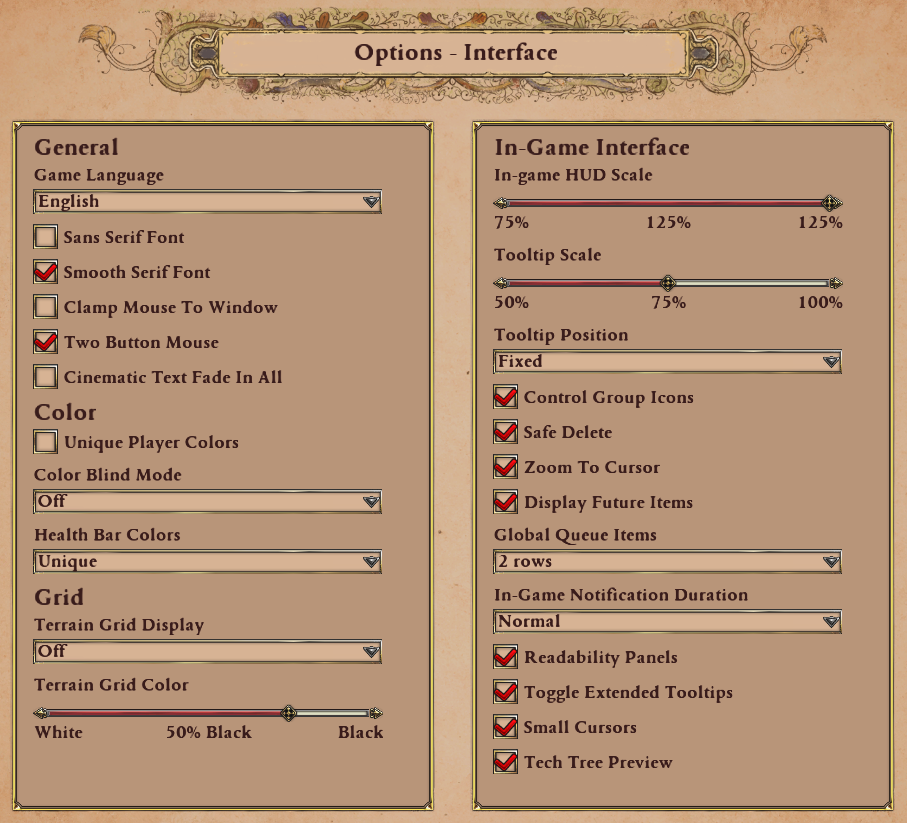
\includegraphics[scale = 0.30]{needed-game-configuration-1.png}
        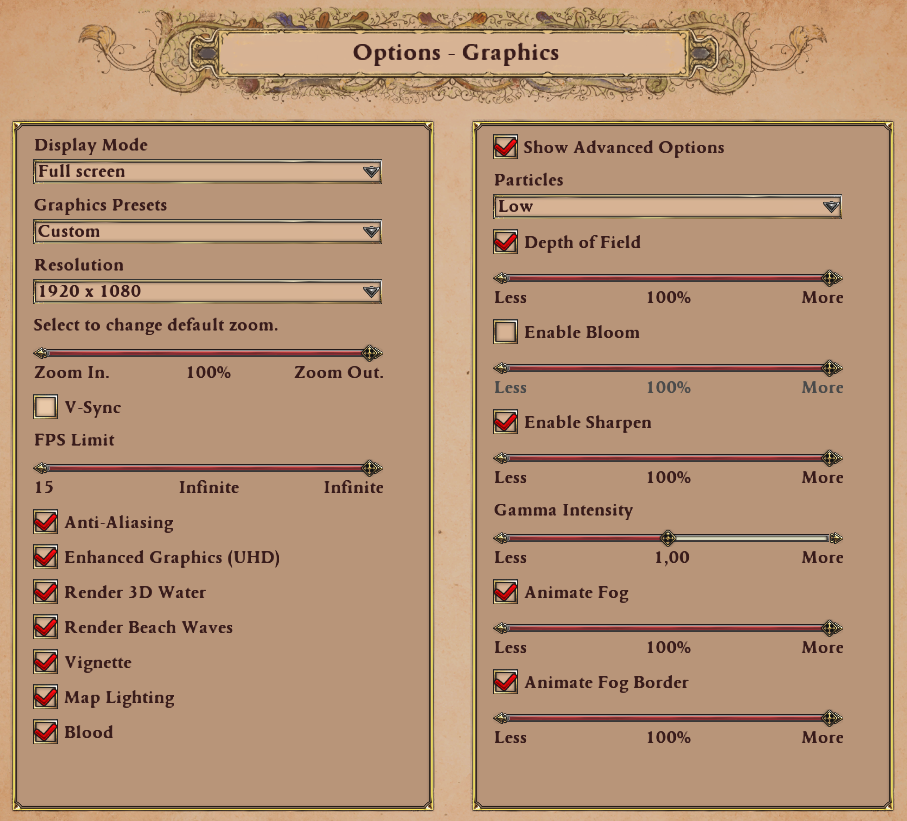
\includegraphics[scale = 0.30]{needed-game-configuration-2.png}
    \end{center}
    \caption{Configuration du jeu requise}
\end{figure}